\documentclass[pdf,table]{beamer}
\usepackage{graphicx,hyperref,pdfpages}
\usepackage{tikz}
\usepackage{textpos}
\usepackage{longtable}
\usetikzlibrary{arrows}
\usetikzlibrary{positioning,chains,fit,shapes,calc}
\usetikzlibrary{mindmap}

\usepackage[style=numeric,backend=biber]{biblatex}
\addbibresource{../CST4025.bib}
\setbeamertemplate{bibliography item}{\insertbiblabel}

\usepackage{listings}
\usepackage{color}
%\usepackage[table]{xcolor}
%\usepackage{booktabs}


\definecolor{codegreen}{rgb}{0,0.6,0}
\definecolor{codegray}{rgb}{0.5,0.5,0.5}
\definecolor{codepurple}{rgb}{0.58,0,0.82}
\definecolor{backcolour}{rgb}{0.95,0.95,0.92}

\lstdefinestyle{mys}{
	backgroundcolor=\color{backcolour},
	commentstyle=\color{codegreen},
	keywordstyle=\color{magenta},
	stringstyle=\color{codepurple},
	numberstyle=\color{codegray},
	basicstyle=\ttfamily\scriptsize,
	breakatwhitespace=false,
	breaklines=true,
	captionpos=b,
	keepspaces=true,
	numbers=left,
	numbersep=5pt,
	showspaces=false,
	showstringspaces=false,
	showtabs=false,
	tabsize=2}
\lstset{style=mys}


\tikzset{every matrix/.style={ampersand replacement=\&,column sep=1.75cm,row sep=2cm},
		BTWMat/.style={ampersand replacement=\&, column sep=0.75cm,row sep=1cm},
		eulerMat/.style={ampersand replacement=\&,column sep=1.1cm,row sep=2cm},
		vertexHighlight/.style={circle,fill=red!80,inner sep=.1cm,text=white},
		vertex/.style={circle,fill=blue!80,inner sep=.1cm,text=white},
		bank/.style={rectangle,fill=blue!50,inner sep=0.1cm,text=black!80}
		edge/.style={--,line width=2pt},
		Dedge/.style={->,line width=2pt},
		DedgeT/.style={->,line width=1pt},
		BiEdge/.style={<->,line width=2pt},
		BiEdgeT/.style={BiEdge,line width=1pt},
		edgeHighlight/.style={--,line width=2pt,color=red},
		loop/.style={min distance=10mm, line width=2pt},
		loopT/.style={min distance=-10mm, line width=1pt},
		label/.style = { rectangle, rounded corners, draw,
		                 minimum width = 2em, fill = yellow!50,
		                 text = red, font = \tiny\bfseries },
		labelT/.style = { circle, draw, line width=1pt,
		                 minimum width = 1em, fill = yellow!50,
		                 text = red, font = \tiny\bfseries },
		every node/.style={align=center}}



\mode<presentation>{
\usetheme{Madrid}
\usecolortheme{beaver}
}


\def\bitcoinA{%
  \leavevmode
  \vtop{\offinterlineskip %\bfseries
    \setbox0=\hbox{B}%
    \setbox2=\hbox to\wd0{\hfil\hskip-.03em
    \vrule height .3ex width .15ex\hskip .08em
    \vrule height .3ex width .15ex\hfil}
    \vbox{\copy2\box0}\box2}}

\newcommand{\cwideadline}{3$^{rd}$ November 2019}
\newcommand{\cwiideadline}{5$^{th}$ January 2020}
%\newcommand{\cwiiideadline}{31$^{st}$ March 2017}
%\newcommand{\cwiiideadline}{15$^{th}$ April 2018}
\newcommand{\resitdeadline}{1$^{st}$ August 2020}
\newcommand{\deferraldeadline}{1$^{st}$ August 2020}
\newcommand{\deferraldeadlineMay}{1$^{st}$ May 2020}
\newcommand{\moduleCode}{CST4025}
\newcommand{\moduleLeader}{Dr Ian Mitchell }
\newcommand{\theauthor}{Dr Ian Mitchell }
\newcommand{\academicyear}{2019-20}
\newcommand{\email}{i.mitchell@mdx.ac.uk}
\newcommand{\moduleTitle}{Blockchain Development}
\newcommand{\office}{T108}
\newcommand{\officehours}{Autumn \& Winter Terms: Tuesdays 1515-1615hrs; and, Wednesdays 1415-1515hrs}
\newcommand{\tel}{0208-411-6014}
\newcommand{\deptName}{Computer Science}
%\newcommand{\officehours}{Friday 1100\--1300hrs Autumn Term \\ Thursday 1400\--1600hrs Winter Term}
%\newcommand{\officehours}{Autumn Term: Mondays 1300\--1500hrs \\ Winter Term: Thursdays 1400\--1600hrs

\def\bitcoinA{%
  \leavevmode
  \vtop{\offinterlineskip %\bfseries
    \setbox0=\hbox{B}%
    \setbox2=\hbox to\wd0{\hfil\hskip-.03em
    \vrule height .3ex width .15ex\hskip .08em
    \vrule height .3ex width .15ex\hfil}
    \vbox{\copy2\box0}\box2}}




\newcommand{\theweek}{1}
\renewcommand{\theequation}{\theweek.\arabic{equation}}

\title[\moduleCode:L\theweek]{\moduleTitle \\ Week: \theweek \\ Title: Blockchain} 

%[\includegraphics[scale=0.2]{../logo/mdxSmall}]
\institute[]{\includegraphics[scale=0.25]{../../../logo/mdxSmall} \\ Middlesex University, \\Dept. of Computer Science, \\London}
\author[\email]{\moduleLeader}
\date{\today}




\begin{document}
	\begin{frame}
		\titlepage
	\end{frame}


\addtobeamertemplate{frametitle}{}{%
\begin{textblock*}{100mm}(.94\textwidth,-0.85cm)
\includegraphics[scale=0.1]{../../../logo/transparent}
\end{textblock*}}

	\begin{frame}{Module Aims}
		\begin{block}{Aims}
	Blockchain Technology is changing how organisations communicate and operate, with this change there is a challenge and opportunity for Blockchain developers. This module aims to convey the required knowledge underpinning blockchain technology in order to enable students to apply it to develop solutions to practical problems.		
		\end{block}
	\end{frame}

	\begin{frame}{Module Objectives}
		\begin{block}{Knowledge}
			\begin{itemize}
				\item {\it Appraise} blockchain types and holistically explain blockchain anatomy
				\item {\it Analyse} a domain specific problem and determine applicatbility of a blockchain solution to that problem
			\end{itemize}	
		\end{block}
		\begin{block}{Skills}
			\begin{itemize}
				\item The design and development of effective blockchain applications
			\end{itemize}
		\end{block}
	\end{frame}


\begin{frame}{Module Syllabus}
	\begin{block}{CST4025: Syllabus}
	\begin{itemize}
		\item  Asynchronous and procedural programming pertaining to blockchain applications
	    	\item  Blockchain data structures for distributed ledger systems
	    	\item  Access Control Language for distributed ledger systems
	    	\item  Implementing business logic for a blockchain solution 
	    	\item  Blockchain and complex system development
	    	\item  Permissioned Blockchain Technologies
	    	\item  Consensus Engineering
	    	\item  Blockchain Engineering
	    	\item  Blockchain Anatomy
	\end{itemize}
	\end{block}
\end{frame}

\begin{frame}{Punctuality, Mobiles and Food}
	\begin{block}{Lateness Policy}
	Please ensure you are on time to sessions as tutors will start sessions promptly.  Please note that if you are more than 15 minutes late you will not be permitted to join the session. 
	\end{block}
	\begin{block}{Mobile Phones}
 Please have your phones on silent throughout the session and only use them in an emergency.
	\end{block}
	\begin{block}{Food \& Drink}
		No eating of food in lab or lecture. \\
		Drinks are permitted in sealed containers. 
	\end{block}
\end{frame}



\begin{frame}{CST4025 \--- Indicative Lecture Plan.}
\begin{table}[tbh!]
\begin{tabular}{ l l}
	Week & Title \\ \hline
	 1 & Introduction to Blockchain\\
	 2 & Composer: Data Modelling\\
	 3 & Composer: Access Control Language\\
	 4 & Formative Feedback \\
	 5 & Asynchronous Programming \& Promises \\ 
	 6 & Composer: Node.js I \\  
	 7 & Composer: Node.js II\\ 
	 8 & Consensus Engineering\\
	 9 & Smart Contracts\\
	 10 & Feedback\\
	 11 & Feedback\\
	 12 &  Presentation\\
 \end{tabular}
	\caption{Lecture Plan, these are indicative titles} 
\end{table}
\end{frame}

\begin{frame}{Administration}
	\begin{columns}[T]
		\begin{column}{0.48\textwidth}
			{\bf Assessment}
			\begin{itemize}
				\item 100\% coursework
					\begin{itemize}
						\item CW1: Data Modelling (25\%)
						\item CW2: Blockchain Development (75\%)
					\end{itemize}
				\item Formative Feedback: Week 4
				\item Formative Feedback: Week 10 \& 11
				\item Presentation: Week 12
				\item e-submission for CW1
				\item hard copy submission for CW2
				\item comply to template
			\end{itemize}
		\end{column}
		\begin{column}{0.48\textwidth}
			{\bf Structure}
			\begin{itemize}
				\item Attendance $>$ 75\%
				\item Resit: \resitdeadline
				\item Deferral: \deferraldeadline
				\item Office: \office
				\item Office Hours: \officehours
				\item Teaching:12 * 2 hour Lab; 12 * 1 hour lecture; 9.5 hours independent study 
				\item Mitigating circumstances: see unihelpdesk and apply for deferral
			\end{itemize}
		\end{column}
	\end{columns}	
\end{frame}


	\begin{frame}{Lecture Aims \& Objectives}
		\begin{itemize}
			\item Introduction to Blockchain
			\item Blockchain Anatomy
			\item centralised vs decentralised
			\item distributed
			\item Consensus
			\item Collaboration
			\item Security
		\end{itemize}
	\end{frame}	

\begin{frame}{What? }
	\begin{block}{Blockchain Definition}
		Append-only immutable distribute ledger forged via consensus on a P2P network
	\end{block}
\end{frame}

\begin{frame}{Where?}
	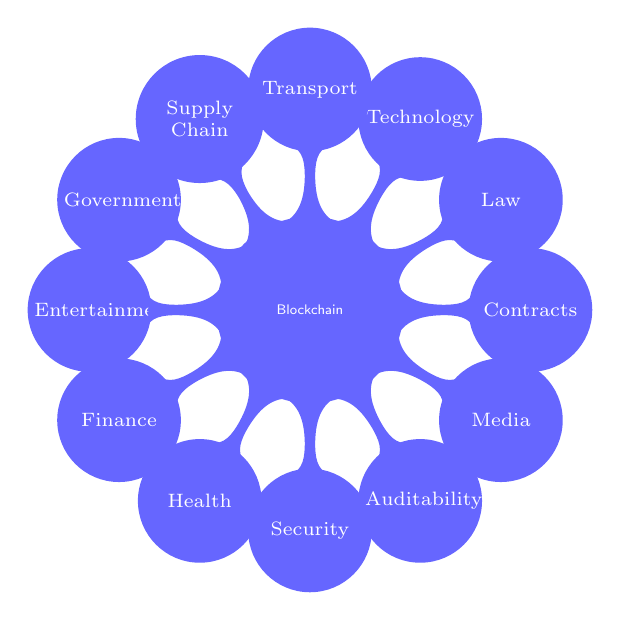
\begin{tikzpicture}[small mindmap, concept color=blue!60, text=white,font=\tiny\sffamily]
\node[concept] {Blockchain}
		child[grow=0] 	{node[concept] {Contracts}}
		child[grow=30] 	{node[concept] {Law}}
		child[grow=60]  {node[concept] {Technology}}
		child[grow=90] 	{node[concept] {Transport}}
		child[grow=120] {node[concept] {Supply Chain}}
		child[grow=150] {node[concept] {Government}}
		child[grow=180] {node[concept] {Entertainment}}
		child[grow=210] {node[concept] {Finance}}
		child[grow=240]	{node[concept] {Health}}
		child[grow=270] {node[concept] {Security}}
		child[grow=300] {node[concept] {Auditability}}
		child[grow=330] {node[concept] {Media}};
\end{tikzpicture}
\end{frame}

\begin{frame}{Blockchain Mindmap}
	\begin{columns}[T]
	\begin{column}{0.6\textwidth}
		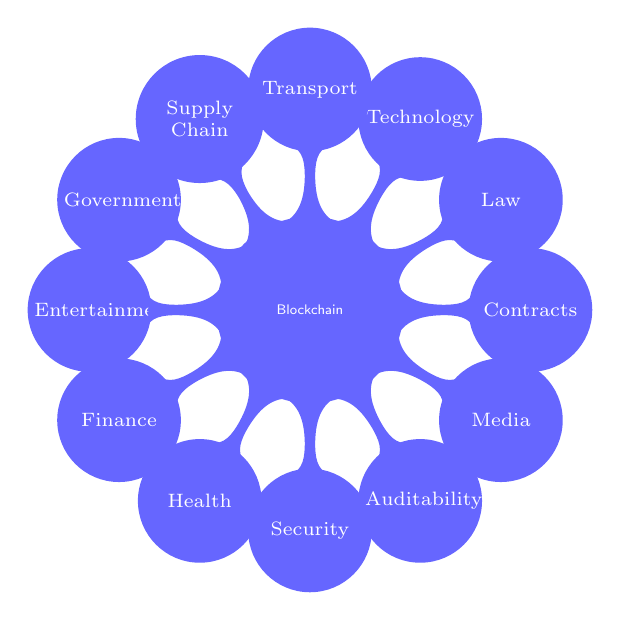
\begin{tikzpicture}[small mindmap, concept color=blue!60, text=white,font=\tiny\sffamily]
		\node[concept] {Blockchain}
		child[grow=0] 	{node[concept] {Contracts}}
		child[grow=30] 	{node[concept] {Law}}
		child[grow=60] 	{node[concept] {Technology}}
		child[grow=90] 	{node[concept] {Transport}}
		child[grow=120] {node[concept] {Supply Chain}}
		child[grow=150] {node[concept] {Government}}
		child[grow=180] {node[concept] {Entertainment}}
		child[grow=210] {node[concept] {Finance}}
		child[grow=240]	{node[concept] {Health}}
		child[grow=270] {node[concept] {Security}}
		child[grow=300] {node[concept] {Auditability}}
		child[grow=330] {node[concept] {Media}};
		\end{tikzpicture}
	\end{column}
	\begin{column}{0.4\textwidth}
		\begin{itemize}
		\item<1|only@1> Contracts
			\begin{itemize}
				\item<1|only@1> Smart Contracts
				\item<1|only@1> Release payment upon satisfying contractual obligations 
				\item<1|only@1> Ratified by using blockchain
			\end{itemize}
		\item<2|only@2> Law
			\begin{itemize}
				\item restriction on dangerous items, e.g. gun control
				\item Police procedures
			\end{itemize}
		\item<3|only@3> Technology
			\begin{itemize}
				\item All areas are seeing blockchain involvement
				\item Fridges, Washing machines, smart environments
				\item Cyber Security
				\item Cloud Storage
				\item Internet of Things, IoT
			\end{itemize}
		\item<4|only@4> Transport
			\begin{itemize}
				\item Public Transportation
				\item Automotive
				\item Business \-- fleets of vehicles and navigation
			\end{itemize}
		\item<5|only@5> Supply Chain
			\begin{itemize}
				\item JIT delivery
				\item Pre-conditions
				\item Smart contracts
				\item Secure
				\item Third party
				\item Mutual (dis)trust
			\end{itemize}
	
		\item<6|only@6> Government
			\begin{itemize}
				\item ID Management
				\item Electoral
				\item Tax
			\end{itemize}

		\item<7|only@7> Entertainment
			\begin{itemize}
				\item Copyright
				\item Digital Rights
			\end{itemize}
		\item<8|only@8> Finance
			\begin{itemize}
				\item Loans
				\item Finance
				\item Business
				\item Reduce Uncertainty
			\end{itemize}
		\item<9|only@9> Health
			\begin{itemize}
				\item Patient records
				\item Patient data
				\item Management and RTW
				\item Private Health sector 
			\end{itemize}
		\item<10|only@10> Security
			\begin{itemize}
				\item blockchain GB
				\item P2P
				\item 4K nodes
				\item 51\% attack 
			\end{itemize}
		\item<11|only@11> Auditability
			\begin{itemize}
				\item UK has many audits
				\item ISO 
				\item QAA - universities
				\item CQC - healthcare
			\end{itemize}
		\item<12|only@12> Media
			\begin{itemize}
				\item Business
				\item share information
				\item immutable history
			\end{itemize}
		\end{itemize}
	\end{column}
\end{columns}
\end{frame}



\begin{frame}{When?}
	\begin{itemize}
		\item \bitcoinA - BitCoin \cite{nakamoto2008bitcoin} 2008
		\item Merkle Trees
		\item Distributed Ledger Technology
		\item Hash algorithms
		\item Crytography
		\item P2P
		\item Consensus Algorithms
	\end{itemize}
\end{frame}


\begin{frame}{How and Why?}
	\begin{itemize}
		\item How, is what \moduleCode is all about
		\item Why, is a little trickier
		\item \url{https://www.youtube.com/watch?v=RplnSVTzvnU}
		\item Reduce uncertainty %Nakamoto was trying the same
	\end{itemize}
\end{frame}


\begin{frame}{Centralised}
     	\begin{itemize}
       		\item Trust
       		\item Governance
       		\item Regulation
       		\item Attributable
       		\item Intermediary
       		\item Transaction Integrity
       	\end{itemize}
\end{frame}



\begin{frame}{Building Blocks}
	\begin{columns}[T]
		\begin{column}{0.45\textwidth}
			\begin{itemize}
				\item Shared append only ledger - immutable database
				\item Cryptography - authentication, integrity \& confidentiality
				\item Consensus - trust and power within the network to verify transactions
				\item Business Logic or smart contracts - rules component of the transaction, e.g., change ownership, update highest bid, etc...
			\end{itemize}
		\end{column}
		\begin{column}{0.50\textwidth}
			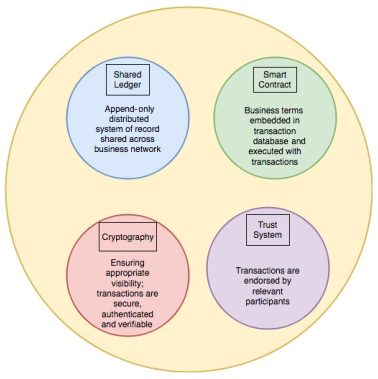
\includegraphics[scale=0.45]{buildingBlocks}
		\end{column}
	\end{columns}	
\end{frame}

\begin{frame}{Other Considerations of blockchain}
	\begin{itemize}
		\item Auditability and logging
		\item Integration: incumbent systems; transaction processing systems; 
		\item Monitoring: quality assurance
		\item Regulations: compliance
		\item Authentication: permissioned and authorised
	\end{itemize}
\end{frame}


\begin{frame}{Blockchain Essentials}
	\begin{columns}[T]
		\begin{column}{0.48\textwidth}
			\begin{itemize}
				\item Merkle trees
				\item Hash
			\end{itemize}
		\end{column}
		\begin{column}{0.48\textwidth}
			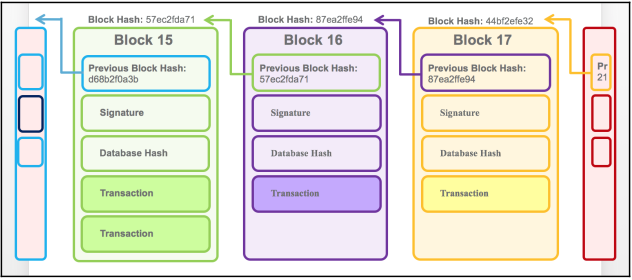
\includegraphics[scale=0.45]{blocks}
		\end{column}
	\end{columns}	
\end{frame}

\begin{frame}{Block Essentials}
	\begin{columns}[T]
		\begin{column}{0.48\textwidth}
			\begin{itemize}
				\item Hashes 
				\item Signature
				\item transaction
				\item unix timestamp
			\end{itemize}
		\end{column}
		\begin{column}{0.48\textwidth}
			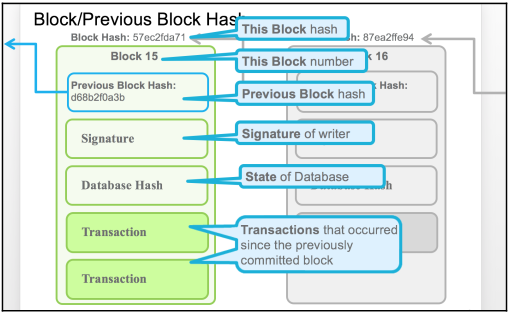
\includegraphics[scale=0.45]{blockEssential}
		\end{column}
	\end{columns}	
\end{frame}

\begin{frame}{Blockchain Essentials}
	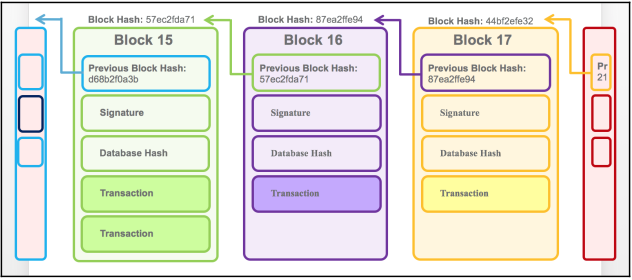
\includegraphics[scale=0.5]{blocks}

\end{frame}

%hyperledger architecture paper 1
\begin{frame}{Hyperledger Architecture \cite{hyperledger:1}}
\begin{itemize}
	\item Consensus 
	\item Smart Contract 
	\item Communication
	\item Data Store
	\item Cryptography
	\item Policy
	\item Identity
	\item API
	\item Interoperation
\end{itemize}
\end{frame}

\begin{frame}{Hyperledger Architecture \cite{hyperledger:1}}
	{\bf Consensus}
\begin{itemize}
	\item Verify the correctness of the set of transactions
	\item A block is composed of multiple transactions
	\item Concur with other nodes
	\item Which of these can be trusted?
	\item Also provides some ordering.
	\item Consensus algorithm:
		\begin{itemize} \pause
			\item Confirms the correctness of transactions in a block, according to the consensus algorithms deployed and the policies applied.
			\item Once the block is confirmed, then it enters the blockchain, so consensus algorithm has to agree on order the blocks are added
			\item Interact and complete smart contract layer 
		\end{itemize}
\end{itemize}
\end{frame}


\begin{frame}{Summary}
	\begin{columns}[T]
		\begin{column}{0.48\textwidth}
			{\bf Blockchain}
			\begin{itemize}
				\item P2P
				\item DLT
					\begin{itemize}
						\item append-only
						\item immutable
						\item hash
						\item signature
						\item blockchain
						\item timestamp
					\end{itemize}
				\item decentralised
				\item trust
			\end{itemize}
		\end{column}
		\begin{column}{0.48\textwidth}
			{\bf Reading}
			\begin{itemize}
				\item NIST \cite{yaga2018blockchain}
				\item Hyperledger \cite{hyperledger:1,hyperledger:2}
				\item Blockchain TED talk by Bettina Warburg (in slides)
			\end{itemize}
		\end{column}
	\end{columns}	
\end{frame}



\begin{frame}[allowframebreaks]{References}
%    	\bibliographystyle{amsalpha}
%	\nocite{hyperledger:gaur2018}          
%	\bibliography{../../../bibliography/forensic2}	
	\printbibliography
\end{frame}
	
\begin{frame}
	\frametitle{Web Resources}
	\begin{itemize}
	\item \url{http://hyperledger.org}
	\end{itemize}
\end{frame}

\end{document}


%\begin{frame}{}
%	\begin{tikzpicture}[]
%	\end{tikzpicture}
%\end{frame}


%\begin{frame}{}
%	\begin{columns}[T]
%		\begin{column}{0.48\textwidth}
%			\begin{lstlisting}
%			\end{lstlisting}
%		\end{column}
%		\begin{column}{0.48\textwidth}
%			{\bf XXX}
%		\end{column}
%	\end{columns}	
%\end{frame}
%
%

%\begin{frame}{}
%	\begin{columns}[T]
%		\begin{column}{0.48\textwidth}
%			\begin{itemize}
%				\item XXX 
%			\end{itemize}
%		\end{column}
%		\begin{column}{0.48\textwidth}
%			{\bf XXX}
%		\end{column}
%	\end{columns}	
%\end{frame}





